\chapter{Teoria della computabilità}
La teoria della computabilità studia quali problemi sono risolvibili utilizzando
una procedura di calcolo meccanica/automatica.
Ragionando in termini più matematici, una funzione $f: I \rightarrow O$
(che altro non è che un problema) è calcolabile sse esiste un algoritmo
che la può calcolare, ovvero che tale che l'algoritmo calcola correttamente,
per ogni $x \in I$, il relativo $f(I)$.

Come si vedrà, non tutti i problemi sono computabili, come l'\textit{halting problem}.

\section{Macchine di Turing}
\subsection{Introduzione alla macchina di Turing}
\subsection*{Cenni storici}
La nozione di algoritmo è stata sempre conosciuta e di facile comprensione:
un algoritmo può essere infatti definito come una sequenza finita e ordinata
di passi che porta, in un tempo finito, al risultato desiderato.
Solo nell'ultimo secolo, però, sono stati definiti dei modelli che
effettivamente descrivono formalmente la nozione di algoritmo.
Queste nuove descrizioni formali sono state sviluppate principalmente per
rispondere al problema della decisione (Entscheidungsproblem), introdotto da
Hilbert nella sua famosa lista di problemi irrisolti al suo tempo nel campo
dei fondamenti della matematica. Il problema chiede se è possibile definire una
procedura automatica che, data una qualsiasi WFF della logica del primo ordine,
stabilisce se la formula è deducibile all'interno della logica del primo ordine,
ovvero è un teorema. Church e Turing hanno risposto negativamente alla domanda,
introducendo rispettivamente il lambda calcolo e le macchine di Turing.

\subsection*{Definizione formale}
Una macchina di Turing, formalmente, è una sestupla:
\begin{center}
    $\ang{\Sigma, \textrm{B}, \textrm{Q}, q_0, \textrm{F}, \delta}$
\end{center}
dove:
\begin{itemize}
    \item $\Sigma$ è l'\textit{alfabeto di nastro}, ovvero l'insieme dei
    simboli che possono essere scritti su nastro. L'alfabeto di nastro è un
    insieme \textit{finito};
    \item B è il \textit{simbolo di blank}, un simbolo speciale usato per
    specificare che una cella del nastro è vuota. Il simbolo di blank
    appartiene all'alfabeto di nastro, ovvero $\textnormal{B} \in \Sigma$;
    \item Q è l'\textit{insieme degli stati} che compongono la FSM.
    L'insieme degli stati è un insieme \textit{finito};
    \item $q_0$ è lo \textit{stato iniziale} della FSM. $q_0$ è uno dei
    possibili stati della FSM, quindi $q_0 \in \textnormal{Q}$;
    \item F è l'\textit{insieme degli stati finali/di accettazione} della FSM.
    Vale $\textnormal{F} \subseteq \textnormal{Q}$;
    \item $\delta$ è la \textit{funzione di transizione}, che definisce come
    avvengono i passaggi di stato della FSM.
\end{itemize}

La parte più “importante” di una macchina di Turing, che di fatto definisce la
sua semantica, è la funzione di transizione.
La funzione di transizione è definita come:
\begin{center}
    $\delta: \textrm{Q} \times \Sigma \rightarrow
    \textrm{Q} \times \Sigma \times \cbra{ \leftarrow, \textrm{\textendash}, \rightarrow }$
\end{center}
ovvero, a partire dallo stato corrente e leggendo il simbolo di nastro puntato
dalla testina, aggiorna lo stato della FSM, scrive nella cella puntata dalla
testina un nuovo simbolo e, infine, muove la testina.

Essendo Q e $\Sigma$ due insiemi finiti, il loro prodotto cartesiano
$\textrm{Q} \times \Sigma$ è un insieme finito, e di conseguenza è possibile
elencare esplicitamente tutti gli elementi del dominio, anche se farlo
effettivamente può richiedere molto tempo e spazio.

Tutte le macchine di Turing sono algoritmi e, viceversa, tutti gli algoritmi
sono macchine di Turing.
Si può così formalizzare la nozione di algoritmo considerandolo, di fatto,
una macchina di Turing.

Si può dire anche che una macchina di Turing è una funzione
\begin{center}
    $f:  \Sigma^* \rightarrow \Sigma^*$
\end{center}
che mappa stringhe su stringhe.

Un sottoinsieme di queste funzioni sono le \textit{funzioni di decisione}:
\begin{center}
    $f: \Sigma^* \rightarrow \{ 0, 1 \}$
\end{center}
Non si perde di generalità considerando solo le funzioni di decisione:
ogni problema generico ha infatti un problema di decisione corrispondente.

Una funzione di decisione può anche essere rappresentata come il linguaggio di
tutte le stringhe per cui la funzione restituisce 1.
\begin{center}
    $L_D = \left\{ x \in \Sigma^* \; | \; f_D (x) = 1 \right\}$
\end{center}
Si può quindi affermare che si ha un'equivalenza tra i problemi (di decisione)
e i linguaggi.

\subsection*{Rappresentazione informale}
Una macchina di Turing può essere vista come una
\textit{macchina a stati finiti} deterministica operante su un \textit{nastro},
diviso in celle, di lunghezza infinita (e quindi memoria infinita);
la macchina possiede, inoltre, una \textit{testina}, che punta ad una singola
cella del nastro.
\begin{figure}[h]
    \centering
    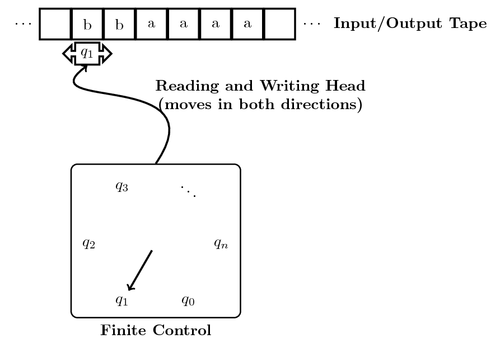
\includegraphics[width=0.5\linewidth]{img/turing_machine.png}
    \caption{Rappresentazione informale della macchina di Turing}
    \label{fig:turing_machine}
\end{figure}

Per convenzione, d'ora in poi si considereranno solo macchine di Turing con
nastro semi-infinito. Non si perde però capacità computazionale:
qualsiasi macchina a nastro infinito può essere simulata con una macchina a
nastro semi-infinito.

\subsection*{Configurazione di una macchina di Turing e complessità}
Lo stato in cui si trova una macchina di Turing a un certo istante di tempo può
essere descritto con la sua \textit{configurazione} (CID), ovvero la quadrupla:
\begin{center}
    $(q, \sigma, \textnormal{sx}, \textnormal{dx})$
\end{center}
dove:
\begin{itemize}
    \item $q$ è lo stato corrente della FSM;
    \item $\sigma$ è il simbolo di nastro presente nella cella puntata dalla
    testina.
    \item sx è il contenuto del nastro a sinistra della testina, quindi dal
    simbolo, diverso dal simbolo di blank, presente più a sinistra alla testina.
    \item dx è il contenuto del nastro a destra della testina, quindi dalla
    testina al simbolo, diverso dal simbolo di blank, più a destra.
\end{itemize}

Una \textit{computazione} della macchina di Turing può quindi essere espressa
come una sequenza di CID.
Il passaggio da una CID alla successiva viene indicato con il simbolo di
derivazione logica $\vdash$.

La computazione di una macchina di Turing può terminare, e quindi essere
rappresentata con una sequenza finita di CID, o non terminare.
Sia $M$ una macchina di Turing e $x$ un input, se la computazione di $M$
su $x$ non termina, allora:
\begin{center}
    $M(x) = \bot$
\end{center}
$\bot$ non è l'output della computazione, ma è solo un simbolo per indicare
la non terminazione della macchina.

Se, invece, la computazione sull'input $x$ termina, allora possono essere
fatte considerazioni sulla sequenza di configurazioni attraversate per arrivare
alla terminazione.

Dato un algoritmo e un input $x$, il numero di configurazioni che la macchina
di Turing che lo modella necessita per terminare viene indicato con $t_M (x)$,
dove $M$ è la macchina di Turing.
Detta $n$ la dimensione dell'input, la \textit{complessità dell'algoritmo}
per input di dimensione $n$ è, invece, il massimo numero di configurazioni che
la macchina può attraversare prima di terminare, dato un input di
dimensione $n$, ed è indicata con $T_M (n)$.
\begin{center}
    $T_M(x) = \textrm{max} \cbra{ t_M(x) \; | \; x \in \textrm{I} \land |x|=n }$
\end{center}
Spesso, però, si è interessati alla sola crescita asintotica della complessità
in funzione della dimensione dell'input, ovvero come varia $T_M (n)$ al
variare di $n$.

L'output di una macchina di Turing che termina varia a seconda della
convenzione adottata: può essere il contenuto del nastro al termine
della computazione (usato per i problemi di ricerca) o lo stato della FSM
al termine della computazione, in particolare YES se ci trova in uno stato
di accettazione, NO altrimenti (usato per i problemi di decisione).

\subsection{Macchina di Turing multinastro}
La macchina di Turing è stata fin'ora definita su un singolo nastro
(semi-infinito).
È però possibile definire una \textit{macchina di Turing multinastro}.
In questo tipo di macchina, la transizione non dipende più, oltre che
dallo stato corrente, da un solo simbolo di nastro: detto $k$ il numero di
nastri, la funzione dipenderà dai $k$ simboli puntati dalle $k$ testine,
una per nastro. Le testine, inoltre, si possono muovere in maniera
completamente indipendente l'una dall'altra.
\begin{figure}[h]
    \centering
    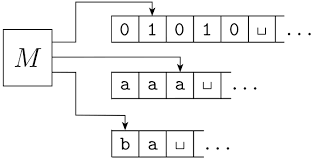
\includegraphics[width=0.5\linewidth]{img/multitape_turing_machine.png}
    \caption{Macchina di Turing multinastro}
    \label{fig:multitape-turing-machine}
\end{figure}
Supponendo di aver assegnato ai $k$ nastri, e di conseguenza alle relative
testine, un indice $1 \le i \le k$, la funzione di transizione per
una macchina multinastro è definita come:
\begin{center}
    $\delta: \textrm{Q} \times \Sigma^k \rightarrow
    \textrm{Q} \times \Sigma^k \times
    \cbra{ \leftarrow, \textrm{\textendash}, \rightarrow }^k$
\end{center}
Una CID è invece definita come:
\begin{center}
    $(q, \sigma^1, \textrm{sx}^1, \textrm{dx}^1, \ldots,
    \sigma^k, \textrm{sx}^k, \textrm{dx}^k)$
\end{center}

\subsection*{Equivalenza tra macchine a singolo nastro e macchine multinastro}
\begin{thm}
    Sia $M$ una macchina di Turing con $k$ nastri, $k>1$, allora esiste $M'$
    macchina di Turing a singolo nastro equivalente, tale che
    $\forall x \in \Sigma^*, \; M(x) = M'(x)$.
\end{thm}

\begin{proof}
    La dimostrazione del teorema è per costruzione. Si vuole dimostrare che:
    \begin{itemize}
        \item data una macchina a singolo nastro, è possibile costruire una
        macchina multinastro che la simula.
        \item data una macchina multinastro, è possibile costruire una
        macchina a singolo nastro che la simula.
    \end{itemize}
    Dimostrare il primo punto è molto semplice: una macchina a singolo nastro
    altro non è che una macchina multinastro con $k = 1$ nastri.
    Di conseguenza, la dimostrazione è già stata fatta.\\
    Il punto critico è poter simulare una macchina multinastro usando una
    macchina a singolo nastro.
    Per farlo, basta semplicemente considerare le stringhe che rappresentano
    lo stato corrente di ognuno dei nastri, e concatenarle usando un nuovo
    carattere separatore, non ancora presente nell'alfabeto di nastro.\\
        INSERIRE IMMAGINE.\\
    Bisogna poter simulare le $k$ testine della macchina multinastro con una
    sola testina. Per farlo, per ogni simbolo $c$ dell'alfabeto di nastro
    della macchina multinastro viene definito il simbolo $\dot{c}$, che
    indica che la cella in cui è contenuto $c$ è puntata dalla testina del
    relativo nastro (simulato).
    Di conseguenza, se $\Sigma$ è l'alfabeto della macchina multinastro e
    $\Sigma'$ l'alfabeto della macchina a singolo nastro:
    \begin{center}
        METTERE RELAZIONE TRA CARDINALITà INSIEMI.
    \end{center}
    Per simulare le transizioni, invece, la macchina a singolo nastro parte
    dall'inizio del nastro (che abbiamo assunto semi-infinito), e scorre il
    nastro fino ad aver letto i $k$ simboli puntati. Durante lo scorrimento,
    però, la macchina deve poter memorizzare i simboli che legge, e lo fa
    usando gli stati della FSM: alla lettura di un particolare simbolo, la
    macchina cambia di stato, di fatto memorizzandolo. Si capisce però che, per
    rappresentare con la FSM tutte le possibili combinazioni degli $n$
    simboli dell'alfabeto della multinastro che è possibile leggere, è
    necessario un numero di stati pari a $|\Sigma|^k$.
    Una volta letti tutti i $k$ simboli puntati, allora la macchina a singolo
    nastro compie la transizione corretta.
\end{proof}

\begin{thm}
    Sia $t_M (x)$ il tempo di calcolo di $M$, macchina di Turing a $k$ nastri,
    $k>1$, e sia $M'$ una macchina a singolo nastro che simula $M$, allora
    \begin{center}
        $t_{M'}(x) = O \bra{t_M(x)} \cdot t_M(x) = O \bra{{t_M (x)}^2}$
    \end{center}
\end{thm}

\begin{proof}
    Sia $s_M (x)$ lo spazio esplorato dalla macchina durante l'esecuzione,
    allora sicuramente $t_M (x) \ge s_M (x)$ (non è infatti possibile visitare
    un numero di celle in un numero di passi inferiore al numero di
    celle stesso).
    Il numero di passi necessari alla macchina a singolo nastro per simulare
    una singola transizione è pari a $O(t_M (x))$: bisogna infatti scorrere
    tutto il nastro simulante fino a leggere tutti i $k$ simboli puntati
    dalle testine simulate, tornare a inizio nastro, scorrere ancora tutto
    il nastro simulato per aggiornare le celle puntate e spostare le testine
    simulate, e infine tornare a inizio nastro.
    Ogni passata richiede $O(t_M(x))$.
    Ma il numero totale di transizioni che la macchina multinastro effettua,
    e quindi il numero di transizioni da simulare, è pari a $t_M(x)$.
    Di conseguenza, il tempo impiegato dalla macchina a singolo nastro per
    simulare il funzionamento della macchina multinastro è pari a:
    \begin{center}
        $t_{M'}(x) = O \bra{{t_M(x)}^2}$
    \end{center}
\end{proof}

\begin{rem}
    I problemi trattabili con una macchina multinastro rimangono trattabili
    anche con una macchina a singolo nastro: sia infatti $t_M(x)$ polinomiale
    in funzione della dimensione dell'input (e quindi trattabile sulla
    macchina multinastro), allora $t_{M'}(x) = O \bra{{t_M(x)}^2}$ è un
    quadrato di un polinomio, che a sua volta è un polinomio.
\end{rem}

\subsection{Macchina di Turing con alfabeto binario}
\begin{thm}
    Sia $M$ una macchina di Turing su alfabeto $\Sigma$, allora esiste $M'$
    con alfabeto $\Sigma' = \cbra{\triangleright, B, 0, 1}$ equivalente.
\end{thm}
\begin{proof}
    La costruzione della macchina $M'$ ad alfabeto binario prevede di
    effettuare la codifica a blocchi dei simboli dell'alfabeto $\Sigma$.
    Ovviamente, per rappresentare un singolo simbolo sarà necessario un
    numero di bit pari a
    $n = \lceil \log_2 |\Sigma \setminus \cbra{ \triangleright, B}| \, \rceil$.
\end{proof}
\begin{rem}
    Il tempo richiesto dalla macchina a codifica binaria $M'$ per simulare
    la macchina $M$ su un input $x$ è
    $t_{M'}(x) = t_M(x) \cdot \lceil \log_2
    |\Sigma \setminus \cbra{\triangleright, B}| \, \rceil$.
    Ma $\lceil \log_2 |\Sigma \setminus \cbra{\triangleright, B}| \, \rceil$
    è costante, e quindi la complessità è:
    \begin{center}
        $t_{M'}(x) = O(t_M(x))$
    \end{center}
\end{rem}

\subsection{Macchina di Turing universale}
La \textit{macchina di Turing universale} è una macchina di Turing che accetta
in input un'altra macchina, codificata come stringa, e un input per la macchina
ricevuta in input.
I computer moderni sono macchine universali, in quanto ricevono in input un
programma (che è la codifica di una macchina di Turing) e un
input per il programma.\\
Per poter descrivere una macchina universale è, però, necessario specificare
come una macchina di Turing può essere codificata tramite una stringa.
Per farlo, basta

FINIRE CODIFICA MACCHINA DI TURING

Tutte le macchine di Turing possono essere codificate sottoforma di stringa e,
viceversa, ogni stringa codifica una macchina di Turing.
Non è però detto che tutte le stringhe portino a una macchina di Turing valida:
sarà compito dell'altra macchina, che la riceverà in input, di
accertarsi di ciò.

\begin{thm}
    Esiste una macchina di Turing $U$, detta macchina di Turing universale,
    tale che,
    $\forall \alpha, x \in \left( \Sigma - \{ \triangleright , B \} \right)^*$,
    si ha $U(\alpha, x) = M_{\alpha} (x)$.
\end{thm}
dove $\alpha$ è la codifica della macchina di Turing a singolo nastro da
simulare, mentre $x$ è l'input per $\alpha$.\\
Per convenzione, se $\alpha$ è la codifica di una macchina di Turing non
valida, allora $U$ si arresta immediatamente.

\begin{proof}
    La dimostrazione viene fatta per costruzione.
    La macchina universale costruita è una multinastro, con $k = 3$, dove:
    \begin{itemize}
        \item il primo nastro coincide con il nastro di $M_{\alpha}$, e
        all'inizio contiene l'input $x$. La testina da simulare coincide
        con la testina di questo nastro;
        \item il secondo nastro contiene lo stato corrente della macchina
        simulata $M_{\alpha}$, più precisamente la codifica dello stato
        corrente. All'inizio conterrà lo stato iniziale di $M_{\alpha}$;
        \item il terzo nastro contiene la codifica $\alpha$.
    \end{itemize}
    \begin{figure}[h]
        \centering
        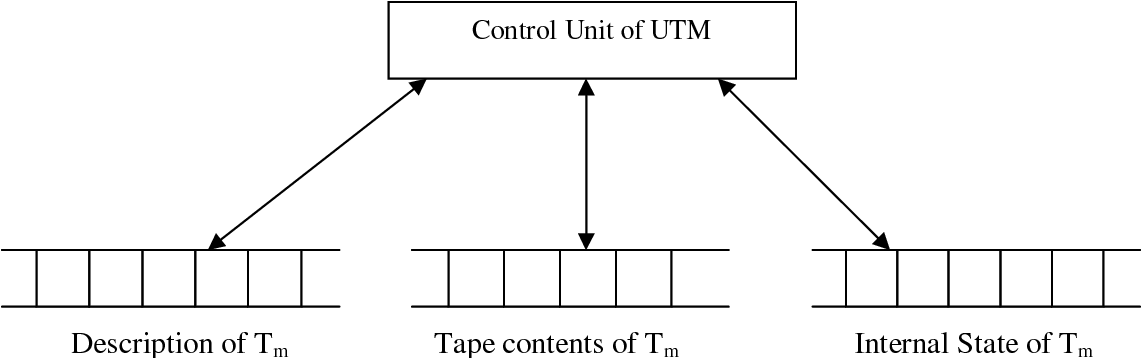
\includegraphics[width=\linewidth]{img/universal_turing_machine.png}
        \caption{Macchina di Turing Universale}
        \label{fig:universal_turing_machine}
    \end{figure}
    Una transizione della macchina $M_{\alpha}$ viene simulata nel
    seguente modo:
    \begin{enumerate}
        \item scorro il terzo nastro (quello della codifica) fino a trovare
        una regola di transizione definita sullo stato corrente $q$,
        contenuto nel secondo nastro.
        \item se ho trovato una regola di transizione sullo stato corrente,
        verifico se essa è definita sullo stesso simbolo di nastro $\sigma$
        puntato dalla testina del primo nastro.\\
        Se ciò è vero, allora è stata trovata la regola di transizione
        corretta, ed è quindi possibile effettuarla: viene quindi copiato
        il nuovo simbolo nella cella puntata dalla testina del primo nastro,
        spostata quest'ultima e, infine, aggiornato lo stato presente sul
        secondo nastro.\\
        Se, invece, il simbolo dettato dalla regola non coincide con quello
        puntato dalla testina del primo nastro, allora si torna al punto 1.
        \item se la macchina universale non riesce a trovare alcuna regola di
        transizione valida per la configurazione corrente della macchina
        simulata, allora la macchina universale termina la sua esecuzione.
    \end{enumerate}
\end{proof}

\begin{thm}
    Sia $t_{M_{\alpha}}(x)$ il tempo di calcolo di $M_{\alpha}$ sull'input $x$,
    e sia $U$ la macchina di Turing universale, che riceve in input la codifica
    $\alpha$ e l'input $x$, allora:
    \begin{center}
        $t_U (\alpha, x) = O \bra{|\alpha| \cdot t_{M_{\alpha}}(x)} =
        O \bra{t_{M_{\alpha}}(x)}$
    \end{center}
\end{thm}

\begin{proof}
    Il tempo di calcolo necessario per simulare una transizione di $M_{\alpha}$
    è pari a $O(1)$: è necessario infatti, per trovare la regola di
    transizione corretta, scorrere solo la codifica $\alpha$, contenuta
    nel terzo nastro della macchina universale, e, di conseguenza, sono
    necessari un numero di passi pari a $O(|\alpha|)$. Ma $|\alpha|$ è
    costante, e quindi $O(|\alpha|) = O(1)$.\\
    Il numero di transizioni da simulare è, invece, pari a $t_{M_{\alpha}}(x)$.
    Di conseguenza,
    $t_U(\alpha, x) = O(1) \cdot t_{M_{\alpha}}(x) = O \bra{t_{M_{\alpha}}(x)}$.
\end{proof}

\begin{rem}
    Se $M_{\alpha}$ è una macchina a singolo nastro, allora la crescita
    asintotica della complessità della macchina universale che la simula,
    in funzione della dimensione $n$ dell'input $x$, è pari a:
    \begin{center}
        $T_U(n) = O \bra{T_{M_{\alpha}}(n)}$
    \end{center}
    I problemi trattabili con una macchina di Turing $M_{\alpha}$ rimangono
    quindi trattabili se $M_{\alpha}$ viene simulata dalla macchina
    universale $U$.
\end{rem}

\subsection{Decidibilità}
Se una macchina di Turing $M$ accetta tutte e sole le stringhe appartenenti
a un linguaggio $L$, allora si dice che $M$ decide $L$.
Non tutti i linguaggi possono essere decisi da una macchina di Turing, e
quindi non tutti i problemi possono essere risolti usando una macchina di
Turing (e quindi un algoritmo): un esempio è l'halting problem.

I problema di decisione (o i rispettivi linguaggi) possono essere
classificati in base alla loro decidibilità:
\begin{itemize}
    \item problemi decidibili (o linguaggi ricorsivi): la relativa macchina
    di Turing termina sempre e fornisce la risposta corretta;
    \item problemi semi-decidibili (o linguaggi ricorsivamente enumerabili):
    la relativa macchina di Turing termina se e solo se l'input $x$ appartiene
    al linguaggio, altrimenti non è garantita la sua terminazione.
    Un esempio di linguaggio semi-decidibile è quello relativo
    all'halting problem.
    \item problemi non decidibili (o linguaggi non ricorsivamente enumerabili):
    non si può garantire che la relativa macchina di Turing termini
    sull'input $x$, sia nel caso $x \in L$ che $x \notin L$.
    Un esempio di linguaggio non ricorsivamente enumerabile è il linguaggio
    di diagonalizzazione.
\end{itemize}
Anche i linguaggi semi-decidibili sono considerati indecidibili da una
macchina di Turing.

Sui linguaggi valgono le seguenti relazioni:
\begin{itemize}
    \item sia $L$ un linguaggio ricorsivo, allora $L$ è ricorsivamente
    enumerabile.
    \item sia $L$ un linguaggio ricorsivo, allora
    $\overline{L} = \cbra{x \in \Sigma^* \; | \; x \notin L}$ è ricorsivo.
    \item $L$ è ricorsivo $\leftrightarrow$ $L$ è ricorsivamente enumerabile
    e $\overline{L}$ è ricorsivamente enumerabile.
\end{itemize}

\subsection{Macchina di Turing non deterministica}
Una macchina di Turing non deterministica è una variante della macchina di
Turing in cui funzione di transizione ammette più regole di transizione per
una stessa coppia stato-simbolo di partenza, e quindi introduce non determinismo
nella scelta della transizione da compiere a partire dallo stato corrente.

La computazione di una macchina di Turing non deterministica può essere
facilmente rappresentata usando un albero di computazione, dove ogni
nodo corrisponde a una configurazione della macchina e ogni
splitting corrisponde alla rappresentazione di tutte le possibili transizioni
valide che è possibile compiere dalla configurazione di splitting.\\
Il grado uscente di una macchina non deterministica è il numero massimo di
configurazioni diverse che possono essere prodotte nel livello $i+1$ a
partire da una singola configurazione nel livello $i$.
\begin{center}
    $r \le |\Sigma_N| \cdot |Q_N| \cdot 3$
\end{center}

Una macchina di Turing non deterministica accetta l'input $x$ sse esiste un
ramo della computazione che accetta $x$.\\
Una macchina di Turing non deterministica rifiuta l'input $x$ sse non esiste
un ramo della computazione che accetta $x$, ovvero tutti i rami rifiutano $x$.\\
In tutti gli altri casi, la macchina di Turing non deterministica non termina.\\
Formalmente, una macchina di Turing accetta quindi un input $x$ sse almeno
uno dei suoi rami termina e accetta $x$, non richiedendo che anche tutti gli
altri rami terminino. Per convenzione, però, verrà assunto che una macchina
di Turing non deterministica accetta $x$ sse almeno un ramo accetta $x$ e
tutti gli altri rami terminano.

\begin{thm}
    Sia $N$ una macchina di Turing non deterministica che accetta il
    linguaggio $L$, allora esiste $D$ macchina di Turing deterministica
    equivalente che accetta $L$.
\end{thm}
\begin{rem}
    Una macchina di Turing non deterministica non ha una capacità
    computazionale maggiore rispetto alla macchina di Turing deterministica.
\end{rem}
\begin{proof}
    Per dimostrare il teorema, bisogna mostrare che una macchina di Turing
    non deterministica può simulare una macchina di Turing deterministica e,
    viceversa, quella deterministica può simulare quella non deterministica.

    Il primo caso è molto semplice: una macchina deterministica può essere
    infatti simulata da una macchina non deterministica usando un solo ramo
    di computazione e nello stesso tempo di calcolo.
    Per quanto riguarda il secondo caso, invece, bisogna ricordare che la
    computazione di una macchina non deterministica definisce un albero delle
    computazioni. Questo albero può essere esplorato usando una visita BFS,
    e questo è quello che farà effettivamente la macchina deterministica per
    compiere la simulazione: utilizzerà quindi una coda, contenente le
    configurazioni correnti della macchina non deterministica, e adotterà
    una politica FIFO per la loro analisi e computazione.

    Non può essere usato l'algoritmo DFS perchè, potendo un ramo della
    macchina non deterministica non terminare, l'algoritmo si potrebbe
    bloccare su rami che non terminano, quando in realtà in rami
    successivi potrebbe essere presente un'accettazione dell'input.
    In questi casi, non si potrebbe quindi garantire l'accettazione di un
    input valido.
\end{proof}

\begin{thm}
    Se la macchina di Turing non deterministica $N$, che decide il
    linguaggio $L$, ha tempo computazionale pari a $T_N (n)$, con $n$
    dimensione dell'input, allora la macchina deterministica $D$ che
    simula $M$ decide $L$ in tempo:
    \begin{center}
        $O\bra{{T_N(x)}^2 \cdot r^{2T_N(n)}}$
    \end{center}
    con $r$ grado uscente massimo di $N$.
\end{thm}
\begin{rem}
    La complessità computazionale della macchina $D$ è pari a un prodotto
    tra un polinomio e una funzione esponenziale: di conseguenza, la
    simulazione effettuata da $D$ risulta inefficiente. Non è quindi garantito
    che problemi trattabili con una macchina di Turing non deterministica
    siano trattabili con la macchina deterministica simulante.
\end{rem}
\begin{proof}
    Il numero $l$ di foglie dell'albero definito dalla computazione di una
    macchina non deterministica $N$ è sicuramente $l \le O(r^{T_N(n)})$, dove
    $O(T_N(n))$ è l'altezza dell'albero e $r$ è il grado uscente della
    macchina non deterministica.
    Lo spazio richiesto dalla macchina di Turing deterministica $D$ per
    simulare una singola foglia è pari alla dimensione del nastro usato
    dal ramo di computazione della macchina non deterministica $N$ associato
    alla foglia.
    Ma, per definizione, il tempo di computazione di un singolo ramo di
    una macchina di Turing non deterministica è polinomiale: di conseguenza,
    anche lo spazio richiesto deve essere polinomiale nella dimensione
    dell'input, ovvero $O(T_N(n))$. Di conseguenza, tutte le configurazioni
    poste nella coda dell'algoritmo BFS avranno dimensione $O(T_N(n))$.
    Lo spazio richiesto per simulare la macchina non deterministica $N$
    usando una macchina deterministica $D$ è quindi pari a
    $O(r^{T_N(n)} \cdot T_N(n))$.

    Per quanto riguarda il tempo di esecuzione della macchina deterministica
    $D$, è stato affermato che la simulazione avviene tramite l'esecuzione
    dell'algoritmo BFS, che esplora l'albero definito dalla computazione
    della macchina non deterministica $N$.
    L'esecuzione dell'algoritmo BFS prevede l'utilizzo di una coda: deve
    infatti essere estratto il primo elemento, rappresentante la
    configurazione che si sta considerando, per poi accodare in fondo alla
    lista tutte le configurazioni raggiungibili dalla configurazione estratta.
    Ma questo implica, per ogni esplorazione di un singolo nodo, di dover
    scorrere la lista due volte: la prima per posizionarsi in fondo alla lista,
    la seconda per tornare alla posizione di partenza.
    La dimensione della coda è $O(r^{T_N(n)} \cdot T_N(n))$.
    Il numero di configurazioni presenti nella coda, e per ognuna della quali
    si deve simulare una transizione, è pari a $O(r^{T_N(n)})$.
    Ma il tempo richiesto per simulare tutte le transizioni da una singola
    configurazione estratta dalla coda è pari a $O(T_N(n))$.
    Di conseguenza, il tempo di esecuzione dell'intero algoritmo BFS è pari a
    $O({T_N(n)}^2 \cdot r^{2T_N(n)})$.
\end{proof}
\begin{rem}
    La dimostrazione per costruzione dimostra che esiste un algoritmo per
    simulare una macchina non deterministica $N$ usando una macchina
    deterministica $D$. Non viene, però, fatta alcuna affermazione sulla
    "qualità" dell'algoritmo, ovvero non viene affermato che esso sia
    effettivamente il migliore. Di conseguenza, il tempo di simulazione
    fornito è solo un upper-bound al possibile tempo di simulazione, da
    parte di una macchina deterministica, di una macchina non deterministica.
    Se si trovasse un algoritmo di simulazione polinomiale, allora P = NP.
\end{rem}

\subsection{Esempi}

\subsection*{Funzione di transizione della macchina che scrive "HELLO"}
FINIRE
La macchina di Turing che deve essere descritta si occuperà di scrivere sul
suo unico nastro la stringa "HELLO".
Il suo alfabeto di nastro è $\Sigma = \{ \triangleright , B, H, E, L, L, O \}$,
mentre il suo nastro è semi-limitato a destra.\\
Il suo funzionamento è molto semplice: scrive infatti H, per poi spostare la
testina a destra e scrivere E, e così via.

$\delta = \left\{
(),
(),
(),
(),
(),
(),
(),
(),
\right\}$

\subsection*{Decidere il linguaggio $\mathbf{a^nb^nc^n}$ con una macchina di
Turing a singolo nastro}
La decisione del linguaggio $a^nb^nc^n$ con una macchina di Turing a singolo
nastro avviene in due fasi: nella prima viene controllato che la stringa di
input abbia struttura $a^*b^*c^*$, mentre la seconda controlla effettivamente
che essa sia nella forma $a^nb^nc^n$.
L'utilizzo della sola seconda fase permetterebbe di accettare stringhe come
$abcabc$, ovviamente non appartenente al linguaggio che si vuole riconoscere.

Fase 1:
\begin{enumerate}
    \item se leggi $a$, continua a leggere le successive $a$
    fino a quando non incontri un simbolo diverso da $a$.\\
    Se questo simbolo è $b$, allora passa al punto 2.\\
    Se questo simbolo è $c$, allora passa al punto 3.\\
    Se questo simbolo è il simbolo di blank, allora passa alla fase 2.
    \item se leggi $b$, continua a leggere le successive $b$ fino a quando
    non incontri un simbolo diverso da $b$.\\
    Se questo simbolo è $a$, allora fallimento.\\
    Se questo simbolo è $c$, allora passa al punto 3.\\
    Se questo simbolo è il simbolo di blank, allora passa alla fase 2.
    \item se leggi $c$, continua a leggere le successive $c$ fino a quando
    non incontri un simbolo diverso da $c$.\\
    Se questo simbolo è il simbolo di blank, allora passa alla fase 2.\\
    In tutti gli altri casi, fallimento.
\end{enumerate}
Fase 2:
\begin{enumerate}
    \item leggi una $a$ e sostituiscila con il simbolo di eliminazione.
    \item cerca a destra una $b$.
    \begin{itemize}
        \item se incontri il simbolo di eliminazione, ignoralo.
        \item se incontri una $c$ o il simbolo di blank, allora fallimento.
        \item se incontri una $b$, sostituiscila con il simbolo di eliminazione
        e passa al punto successivo.
    \end{itemize}
    \item cerca a destra una $c$.
    \begin{itemize}
        \item se incontri il simbolo di eliminazione, ignoralo.
        \item se incontri il simbolo di blank, allora fallimento.
        \item se incontri una $c$, sostituiscila con un simbolo di eliminazione
        e passa al punto successivo.
    \end{itemize}
    \item riposiziona la testina a inizio nastro.
    \item se sono presenti $a$ non lette, torna al punto 1.
    Altrimenti, scorri il nastro fino ad incontrare il primo simbolo di blank.
    \begin{itemize}
        \item se incontri il simbolo di eliminazione, ignoralo.
        \item se incontri $b$ o $c$, allora fallimento.
        \item se incontri il simbolo di blank, allora successo.
    \end{itemize}
\end{enumerate}


\subsection*{Decidere il linguaggio $\mathbf{a^nb^nc^n}$ con una macchina di
Turing multinastro SISTEMARE ITALIANO}
Un esempio di risoluzione di un problema tramite una macchina deterministica
multinastro riguarda il linguaggio $a^nb^nc^n$.
Si vuole verificare che la stringa di input scritta sul nastro abbia
effettivamente questa struttura, e per farlo si usa una macchina multinastro
con 3 nastri.
Un algoritmo potrebbe essere il seguente:
\begin{enumerate}
    \item la stringa di input viene posta sul primo nastro. Secondo e terzo
    nastro sono vuoti.
    \item controlla che l'input sia della forma $a^*b^*c^*$. Per farlo,
    la macchina scorre semplicemente il primo nastro.
    Se l'input non è valido, allora si ha un fallimento.
    \item si posizionano tutte le testine dei nastri a inizio nastro.
    \item si legge il simbolo puntato dalla testina del primo nastro:
    \begin{itemize}
        \item se $a$, allora lo si ignora.
        \item se $b$, allora lo si sposta sul secondo nastro.
        \item se $c$, allora lo si sposta sul terzo nastro.
    \end{itemize}
    Dopo aver letto un simbolo, la testina del primo nastro viene spostata a
    destra, ed eventualmente anche la testina del nastro su cui si è spostato
    il simbolo viene spostata a destra.
    \item esegue il punto precedente fino a quando tutta la stringa di input
    (primo nastro) è stata letta.
    \item riposiziona tutte le testine agli inizi dei rispettivi nastri.
    \item legge i simboli puntati dalle 3 testine:
    \begin{itemize}
        \item se la prima testina punta a una $a$, la seconda a $b$ e la terza
        a $c$, allora sposta tutte le testine a destra e ripete questo punto.
        \item se i simboli puntati sono tutti il simbolo di blank, allora la
        stringa di input è della forma $a^nb^nc^n$. La macchina quindi termina
        con successo.
        \item in tutti gli altri casi, la stringa di input non è della forma
        $a^nb^nc^n$. La macchina quindi termina con fallimento.
    \end{itemize}
\end{enumerate}

\begin{rem}
    Il tempo richiesto dalla macchina di Turing a singolo nastro per
    verificare se una stringa appartiene al linguaggio $a^nb^nc^n$ è pari a
    $O(m^2)$, con $m$ lunghezza della stringa.
\end{rem}
